\documentclass[]{article}
\usepackage{lmodern}
\usepackage{amssymb,amsmath}
\usepackage{ifxetex,ifluatex}
\usepackage{fixltx2e} % provides \textsubscript
\ifnum 0\ifxetex 1\fi\ifluatex 1\fi=0 % if pdftex
  \usepackage[T1]{fontenc}
  \usepackage[utf8]{inputenc}
\else % if luatex or xelatex
  \ifxetex
    \usepackage{mathspec}
  \else
    \usepackage{fontspec}
  \fi
  \defaultfontfeatures{Ligatures=TeX,Scale=MatchLowercase}
\fi
% use upquote if available, for straight quotes in verbatim environments
\IfFileExists{upquote.sty}{\usepackage{upquote}}{}
% use microtype if available
\IfFileExists{microtype.sty}{%
\usepackage{microtype}
\UseMicrotypeSet[protrusion]{basicmath} % disable protrusion for tt fonts
}{}
\usepackage[margin=1in]{geometry}
\usepackage{hyperref}
\hypersetup{unicode=true,
            pdftitle={Expanding ggplot2 for better visual exploration of missing data},
            pdfauthor={Nicholas Tierney, Dianne Cook, Monash University},
            pdfborder={0 0 0},
            breaklinks=true}
\urlstyle{same}  % don't use monospace font for urls
\usepackage{color}
\usepackage{fancyvrb}
\newcommand{\VerbBar}{|}
\newcommand{\VERB}{\Verb[commandchars=\\\{\}]}
\DefineVerbatimEnvironment{Highlighting}{Verbatim}{commandchars=\\\{\}}
% Add ',fontsize=\small' for more characters per line
\usepackage{framed}
\definecolor{shadecolor}{RGB}{248,248,248}
\newenvironment{Shaded}{\begin{snugshade}}{\end{snugshade}}
\newcommand{\KeywordTok}[1]{\textcolor[rgb]{0.13,0.29,0.53}{\textbf{{#1}}}}
\newcommand{\DataTypeTok}[1]{\textcolor[rgb]{0.13,0.29,0.53}{{#1}}}
\newcommand{\DecValTok}[1]{\textcolor[rgb]{0.00,0.00,0.81}{{#1}}}
\newcommand{\BaseNTok}[1]{\textcolor[rgb]{0.00,0.00,0.81}{{#1}}}
\newcommand{\FloatTok}[1]{\textcolor[rgb]{0.00,0.00,0.81}{{#1}}}
\newcommand{\ConstantTok}[1]{\textcolor[rgb]{0.00,0.00,0.00}{{#1}}}
\newcommand{\CharTok}[1]{\textcolor[rgb]{0.31,0.60,0.02}{{#1}}}
\newcommand{\SpecialCharTok}[1]{\textcolor[rgb]{0.00,0.00,0.00}{{#1}}}
\newcommand{\StringTok}[1]{\textcolor[rgb]{0.31,0.60,0.02}{{#1}}}
\newcommand{\VerbatimStringTok}[1]{\textcolor[rgb]{0.31,0.60,0.02}{{#1}}}
\newcommand{\SpecialStringTok}[1]{\textcolor[rgb]{0.31,0.60,0.02}{{#1}}}
\newcommand{\ImportTok}[1]{{#1}}
\newcommand{\CommentTok}[1]{\textcolor[rgb]{0.56,0.35,0.01}{\textit{{#1}}}}
\newcommand{\DocumentationTok}[1]{\textcolor[rgb]{0.56,0.35,0.01}{\textbf{\textit{{#1}}}}}
\newcommand{\AnnotationTok}[1]{\textcolor[rgb]{0.56,0.35,0.01}{\textbf{\textit{{#1}}}}}
\newcommand{\CommentVarTok}[1]{\textcolor[rgb]{0.56,0.35,0.01}{\textbf{\textit{{#1}}}}}
\newcommand{\OtherTok}[1]{\textcolor[rgb]{0.56,0.35,0.01}{{#1}}}
\newcommand{\FunctionTok}[1]{\textcolor[rgb]{0.00,0.00,0.00}{{#1}}}
\newcommand{\VariableTok}[1]{\textcolor[rgb]{0.00,0.00,0.00}{{#1}}}
\newcommand{\ControlFlowTok}[1]{\textcolor[rgb]{0.13,0.29,0.53}{\textbf{{#1}}}}
\newcommand{\OperatorTok}[1]{\textcolor[rgb]{0.81,0.36,0.00}{\textbf{{#1}}}}
\newcommand{\BuiltInTok}[1]{{#1}}
\newcommand{\ExtensionTok}[1]{{#1}}
\newcommand{\PreprocessorTok}[1]{\textcolor[rgb]{0.56,0.35,0.01}{\textit{{#1}}}}
\newcommand{\AttributeTok}[1]{\textcolor[rgb]{0.77,0.63,0.00}{{#1}}}
\newcommand{\RegionMarkerTok}[1]{{#1}}
\newcommand{\InformationTok}[1]{\textcolor[rgb]{0.56,0.35,0.01}{\textbf{\textit{{#1}}}}}
\newcommand{\WarningTok}[1]{\textcolor[rgb]{0.56,0.35,0.01}{\textbf{\textit{{#1}}}}}
\newcommand{\AlertTok}[1]{\textcolor[rgb]{0.94,0.16,0.16}{{#1}}}
\newcommand{\ErrorTok}[1]{\textcolor[rgb]{0.64,0.00,0.00}{\textbf{{#1}}}}
\newcommand{\NormalTok}[1]{{#1}}
\usepackage{graphicx,grffile}
\makeatletter
\def\maxwidth{\ifdim\Gin@nat@width>\linewidth\linewidth\else\Gin@nat@width\fi}
\def\maxheight{\ifdim\Gin@nat@height>\textheight\textheight\else\Gin@nat@height\fi}
\makeatother
% Scale images if necessary, so that they will not overflow the page
% margins by default, and it is still possible to overwrite the defaults
% using explicit options in \includegraphics[width, height, ...]{}
\setkeys{Gin}{width=\maxwidth,height=\maxheight,keepaspectratio}
\IfFileExists{parskip.sty}{%
\usepackage{parskip}
}{% else
\setlength{\parindent}{0pt}
\setlength{\parskip}{6pt plus 2pt minus 1pt}
}
\setlength{\emergencystretch}{3em}  % prevent overfull lines
\providecommand{\tightlist}{%
  \setlength{\itemsep}{0pt}\setlength{\parskip}{0pt}}
\setcounter{secnumdepth}{0}
% Redefines (sub)paragraphs to behave more like sections
\ifx\paragraph\undefined\else
\let\oldparagraph\paragraph
\renewcommand{\paragraph}[1]{\oldparagraph{#1}\mbox{}}
\fi
\ifx\subparagraph\undefined\else
\let\oldsubparagraph\subparagraph
\renewcommand{\subparagraph}[1]{\oldsubparagraph{#1}\mbox{}}
\fi

%%% Use protect on footnotes to avoid problems with footnotes in titles
\let\rmarkdownfootnote\footnote%
\def\footnote{\protect\rmarkdownfootnote}

%%% Change title format to be more compact
\usepackage{titling}

% Create subtitle command for use in maketitle
\newcommand{\subtitle}[1]{
  \posttitle{
    \begin{center}\large#1\end{center}
    }
}

\setlength{\droptitle}{-2em}
  \title{Expanding ggplot2 for better visual exploration of missing data}
  \pretitle{\vspace{\droptitle}\centering\huge}
  \posttitle{\par}
  \author{Nicholas Tierney, Dianne Cook, Monash University}
  \preauthor{\centering\large\emph}
  \postauthor{\par}
  \predate{\centering\large\emph}
  \postdate{\par}
  \date{15/12/2016}


\begin{document}
\maketitle

\section{Introduction}\label{introduction}

Missing data is ubiquitous in data analysis. Existing approaches to
exploring missing data structure provide stand alone software, or build
their own workflow inside R. ggplot2, an implementation of the grammar
of graphics is an incredibly popular way to produce data visualisations
does not currently support missing data. Tidy data format (Wickham 2014)
states that each row is an observation and each column is a variable,
which makes it easy and consistent to perform data manipulation and
wrangling. There are currently no guidelines for representing additional
missing data structures in a tidy format. This paper describes
approaches for exploring missing data structure with minimal deviation
from the common workflows of ggplot and tidy data structures. We first
describe typical sources of missing data, seribe existing software for
handling missing data, we then go on to explain data structures for
missing data, visulisations and numerical summaries for missing data,
and then discuss the impact of these methods, the current limitations,
and future plans.

\section{Types of missing data}\label{types-of-missing-data}

Canonical sources of missing data are questionnaires. Data obtained from
questionnaires are often subject to both unknown and known missingness
structure. Unknown missing data structure may arise from respondents
accidentally failing to answer questions or inadvertently providing
inappropriate answers. Known missing data structure data may arise due
to the structure of the questionnaire. For example, the first question
on a survey might be: `If YES, skip to question 4', resulting in
questions 2 and 3 missing. If the structure of the questionnaire is
known, this type of missingness can be evaluated easily. However, if
this information is not available, the mechanism responsible for
producing missing data must be inferred from the data. Longitudinal
studies are also sources of missing data, where participants may not
return for future testing sessions. In these cases it is difficult,
sometimes impossible, to ascertain the reason for the dropouts, and
hence, whether the missingness structure is known or unknown.

There are a two main approaches to analysis of data with missing values,
deletion and imputation. The first approach is deletion, where
variables, or cases may be dropped depending on the amount of missing
data. It is now widely regarded as best practice to instead impute these
values, replacing the missing values with some other value estimated
from the data (Schafer and Graham 2002). In order for estimates to be
unbiased, it is essential to understand the missingness structure and
mechanisms (Little 1988; Rubin 1976; Simon and Simonoff 1986).

\subsection{Existing packages for handling missing
data}\label{existing-packages-for-handling-missing-data}

Software focussing on missing data typically focus on imputation or
visualisation. Packages such as mice, Hmisc, mi, Amelia, and mitools
provide functions to facilitate imputation, and use a wide range of
methods, from mean or median imputation, to regression or machine
learning, to Bayesian methodologies {[}({\textbf{???}});
({\textbf{???}}); etc. {]}. Packages typically provide approaches for
aggregating and evaluating imputations. Maintaining a consistent data
structure when These packages provide a wide variety of different
imputation methods, with more work from new packages such as
\texttt{simputation} ({\textbf{???}}) using the pipe
\texttt{\%\textgreater{}\%} operator with imputation procedures and
working with the \texttt{dplyr} data manipulation. It is again important
to take care to avoid bias when performing multiple imputation.

Missing data visualisation packages include the R package VIM, and the
stand alone softwares MANET, ggobi, and MissingDataGUI (Cheng et al.
2015; Unwin et al. 1996; Swayne et al. 2003; Templ et al. 2011). MANET
(Missings Are Now Equally Treated), provides univariate visualisations
of missing data using linked brushing between a reference plot of the
missingness for each variable, and a plot of the data as a histogram or
barplot. ggobi extends the univariate linked brushing of MANET to
multivariate, using parallel co-ordinate plots. ggobi also provided
incoporated missingness into scatterplots, displaying missing values
from one variable as 10\% below the minimum value on the other axis.
MissingDataGUI provides a user interface for exploring missing data
structure both numerically and visually. A limitation of these softwares
are that being stand alone software packages breaks workflow from
statistical analysis. Although using a GUI to explore missing data may
provide some valuable insights into important structures, it can then be
hard to incorporate these unscripted insights into reproducible
analyses.

VIM (Visualising and Imputing Missing Data) is an R package that
provides methods for both imputation and visualisation of missing data.
In particular it provides visualisations that identify observed,
imputed, and missing values. VIM also identifies imputed cases by adding
a suffix to a variable, so Var1 would have a sibling indicator column,
Var1\_imp, where each case is TRUE or FALSE to indicate imputed or not.
Although VIM provides R functions to visualise and impute missing data,
it's syntax for data manipulation and visualisation is difficult to
extend, and as a result can be difficult to keep in a tidy framework.
ggplot2, an implementation of Lee Wilkenson's grammer of graphics in R
(very popular), currently only provides visualisation of missing values
for categories when there is a category variable, this provides
visualisations for missing data when the values being plotted are
categories, it treats one of the categories as a NA value. For all other
plots, ggplot2 prints a warning message notifying the user how many
missing values have been ommited form the plot.

We see that there are many ways to explore missing data structure and
imputation, however there is no unified methodology or approach to
representing data structures, imputing values, and visualising missing
data structure. We now discuss how we can represent missing data in
particular data structures that align themselves with a tidy data
workflow.

\section{Data structures for missing
data}\label{data-structures-for-missing-data}

Representing missing data structure is achieed using the shadow matrix,
introduced in Swayne and Buja Swayne and Buja (1998; 1998). The shadow
matrix is the same dimension as the data, and consists of binary
indicators of ``missingness'' of data values. In our case, missing is
represented as ``NA'', and not missing is represented as ``!NA'',
although these may be represented as 1 and 0, respectively. This can be
seen in figure 1 below. This structure can also be extended to allow for
additional factor levels to be created, where 0 indicates presence, 1
indicates missing, 2 might indicate an imputed value, or 3 might
indicate a particular type or class of missingness - perhaps missing due
to a particular reason.

\begin{figure}[h]
\centering
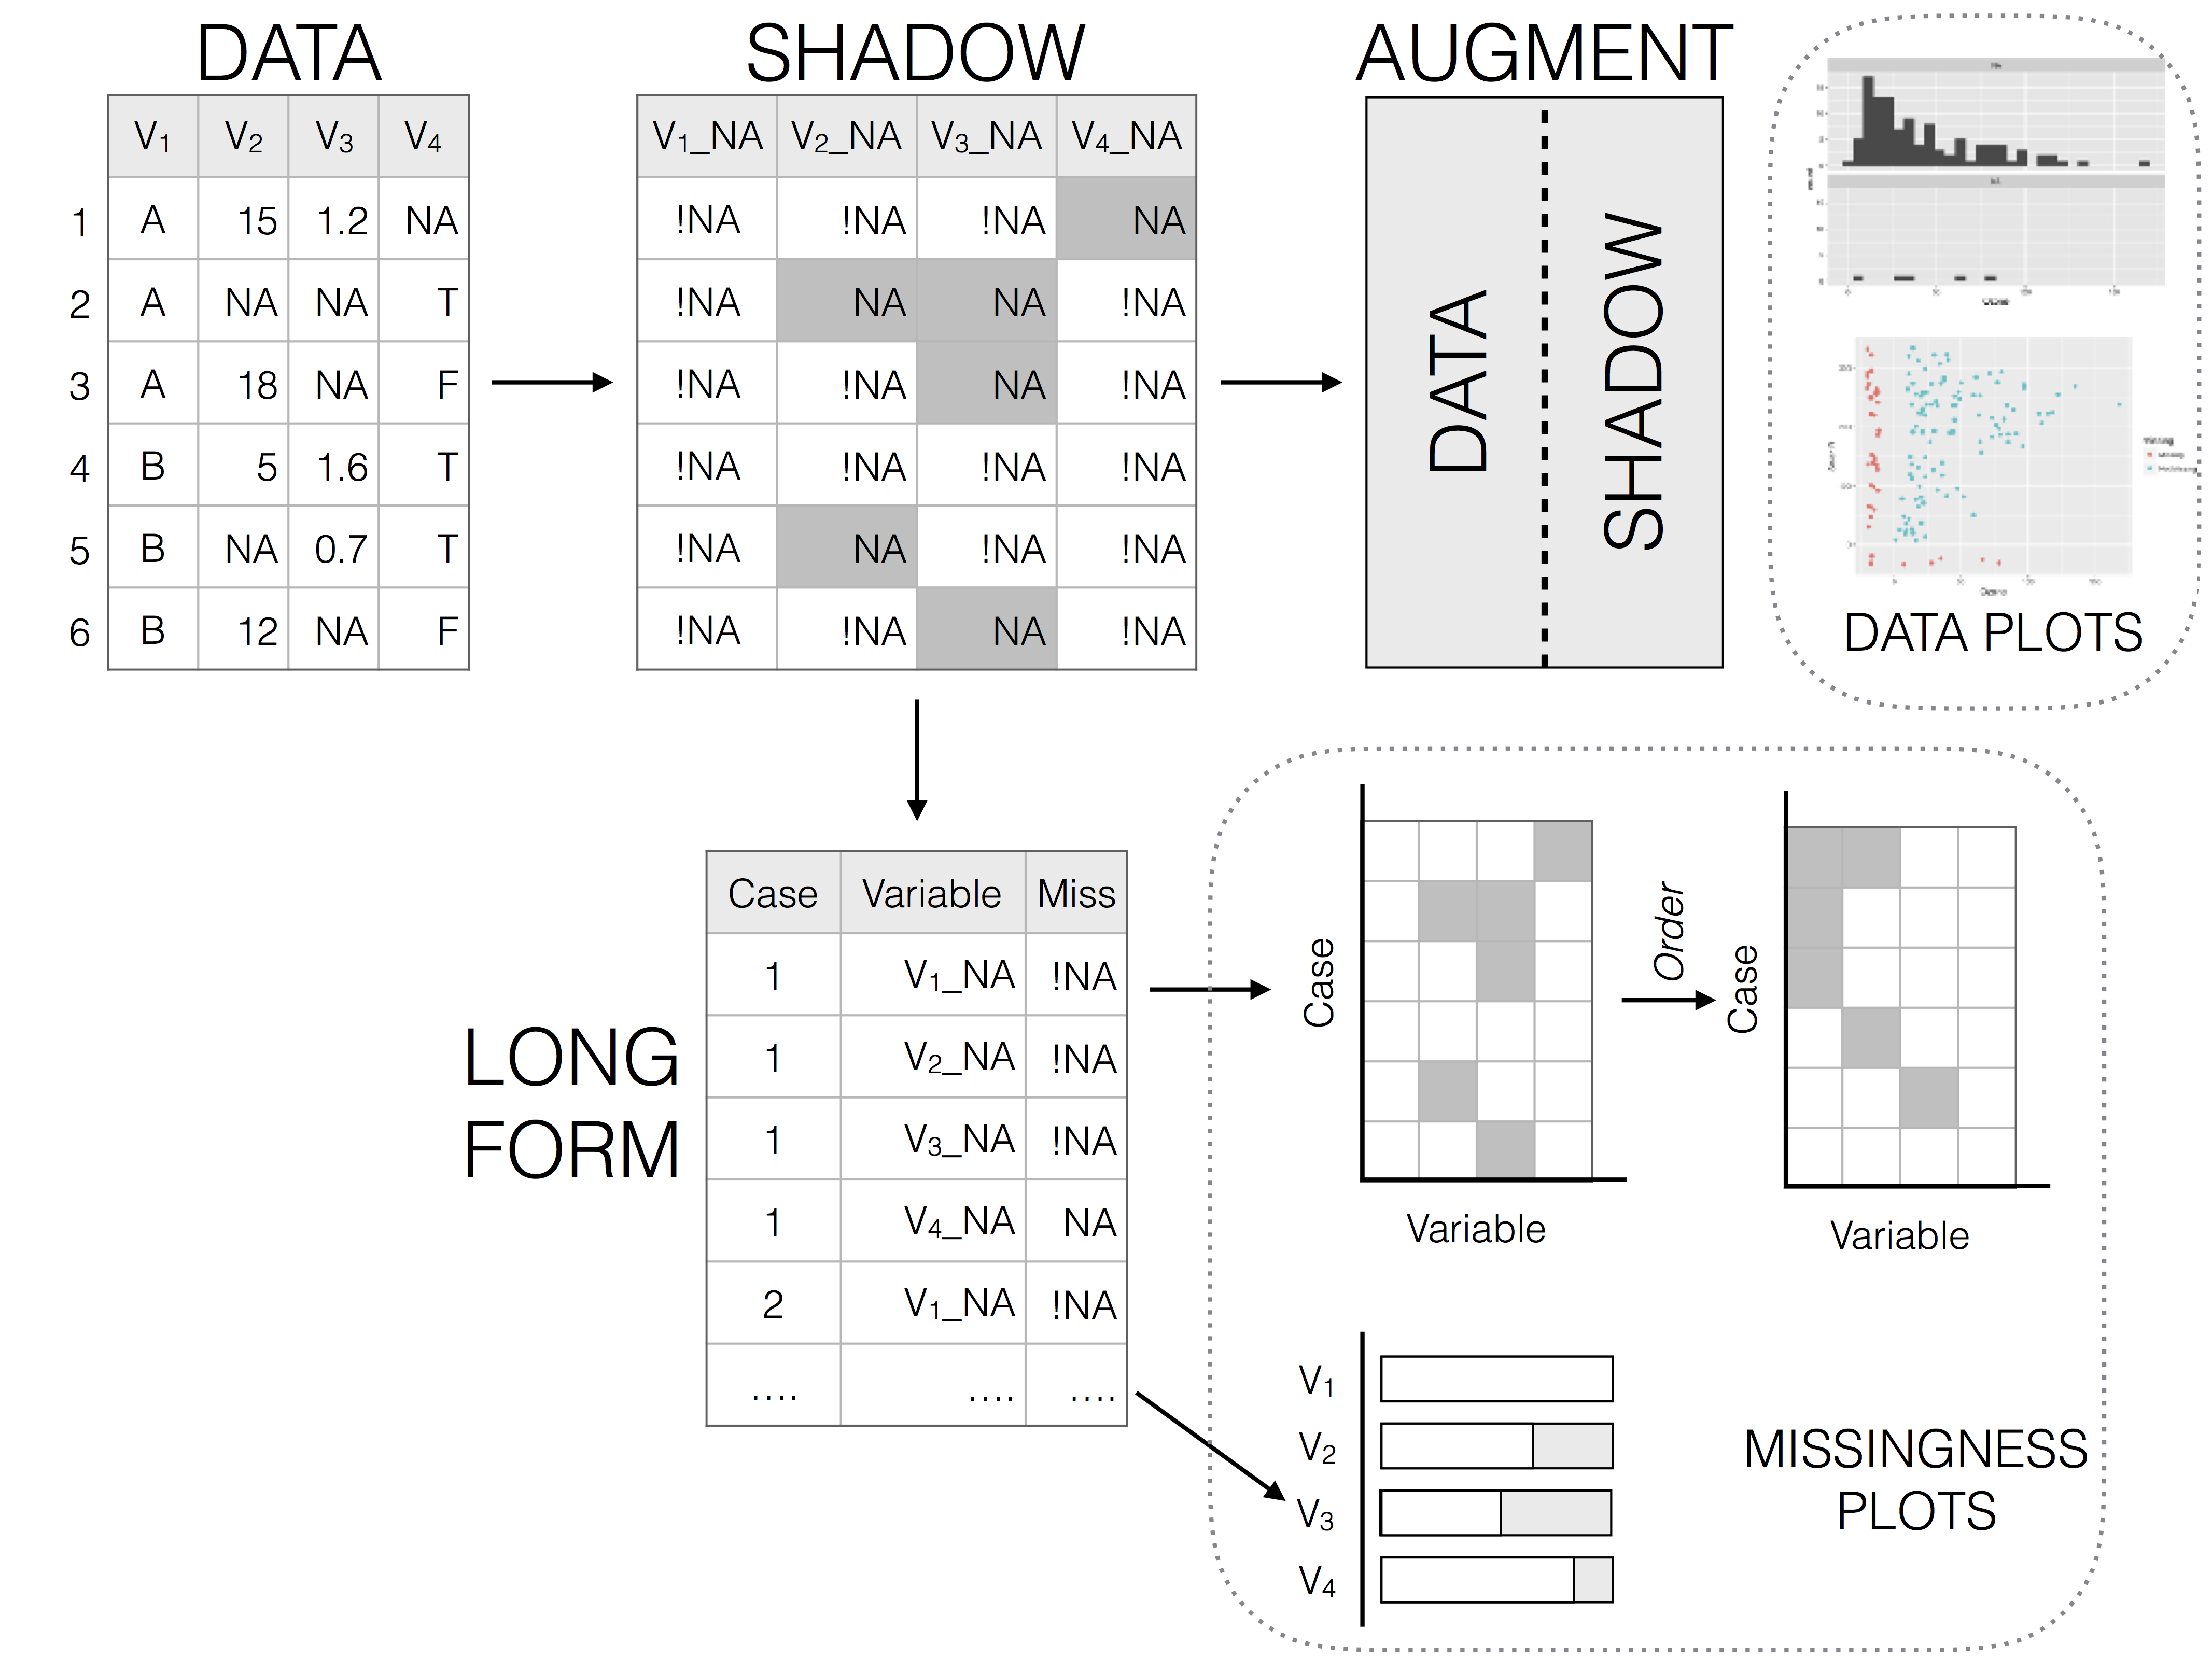
\includegraphics[width=270pt]{/Users/tierneyn/Google Drive/ALL THE THINGS/PhD/code/R/jsm2017/diagram.png}
\end{figure}

The shadow matrix is represented in figure 1 going from Data to Shadow
to show the existing datastructure, adding the suffix ``\_NA" to the
variables. The data matrix can be augmented to include the shadow
matrix, which facilitates visualisation of univariate and bivariate
missing data visualisations. Another format is to display it in long
form, which facilitates heatmap type visualisations of missing data.

\subsection{Visualising missing data}\label{visualising-missing-data}

\textbf{Heatmap}

One common method for visualising missing data is to display a heatmap
of the shadow matrix. This approach can be very helpful for giving an
overview of which variables contain the most missingness. Methods can
also be applied to rearrange rows and columns to find clusters, and
identify other interesting features of the data that may have previously
been hidden or unclear. This method is shown below using the
\texttt{vis\_miss} command from the \texttt{visdat} package.

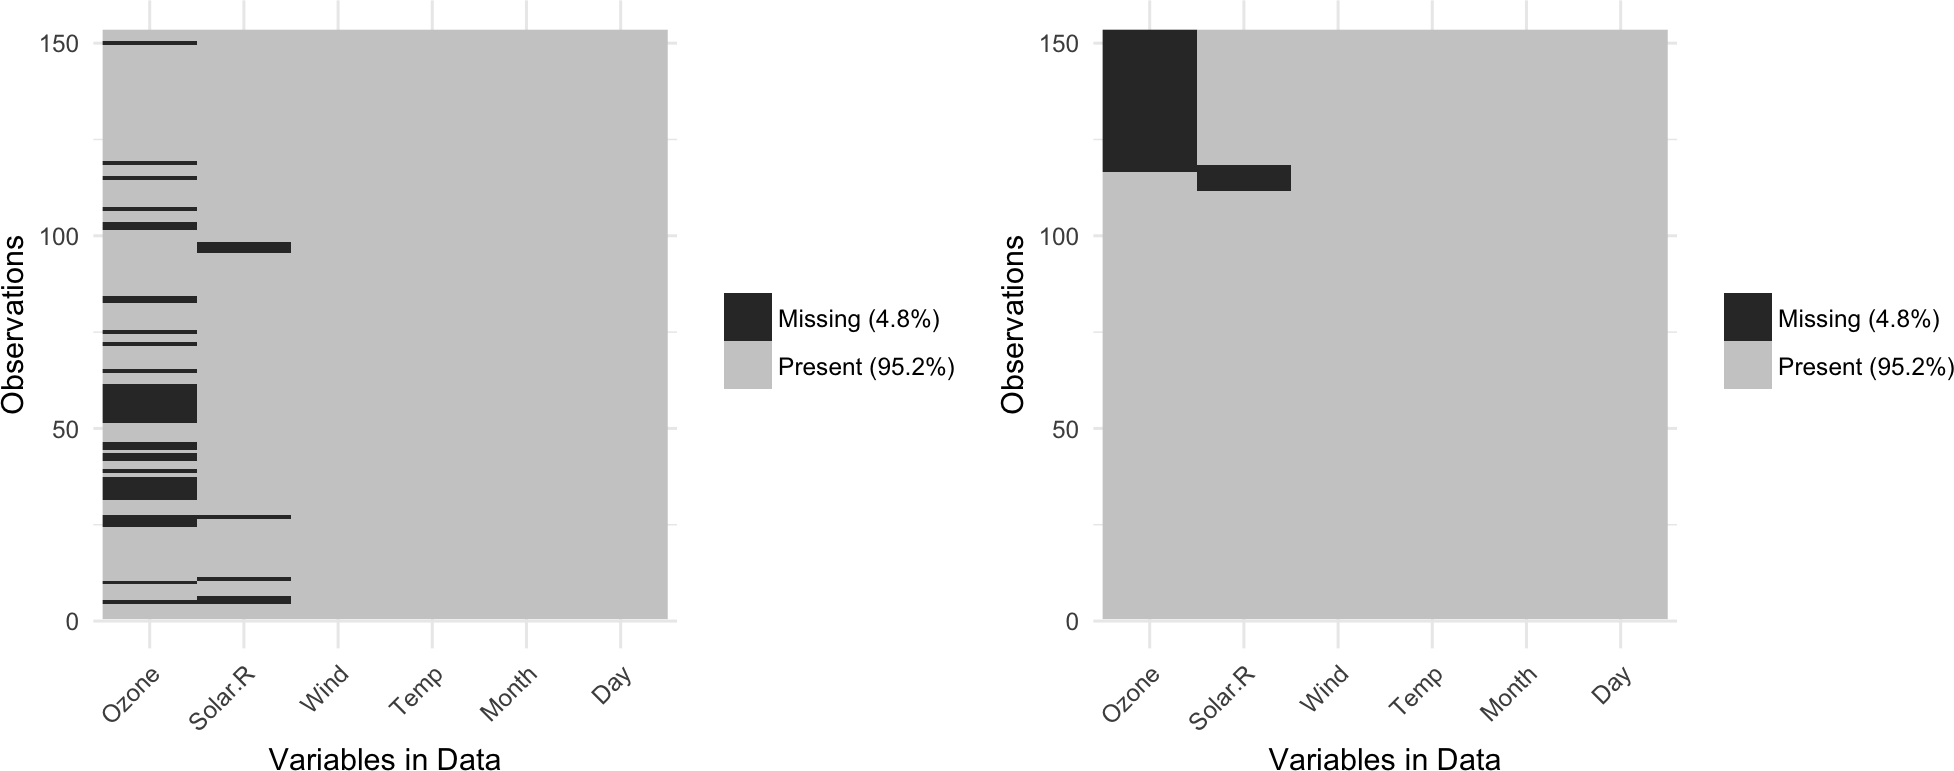
\includegraphics{jsm2017_files/figure-latex/unnamed-chunk-1-1.png}

Similar approaches have been used in other missing data packages such as
VIM, mi, Amelia, and MissingDataGUI. However this plot provides the
additional benefits of being in the ggplot framework, which gives users
greater control over the plot appearance, and alter and update the
figure as they need. The user can also apply clustering of the rows and
columns using the \texttt{cluster\ =\ TRUE} argument.

\textbf{Facetted plots}

An advantage of the wide shadow format is that it allows for referring
to missingness of other variables along the values of another variable.
For example, we an explore the values of when Solar.R is present and
missing. The density plot shows both missing and not missing Solar.R in
one plot, but the histogram shows that there really aren't many values
of Ozone that are missing.

\begin{verbatim}
ggplot(data = bind_shadow(airquality),
       aes(x = Ozone)) + 
  geom_histogram() + 
  facet_wrap(~Solar.R_NA,
             ncol = 1)

ggplot(data = bind_shadow(airquality),
       aes(x = Ozone,
           colour = Solar.R_NA)) + 
  geom_density()
\end{verbatim}

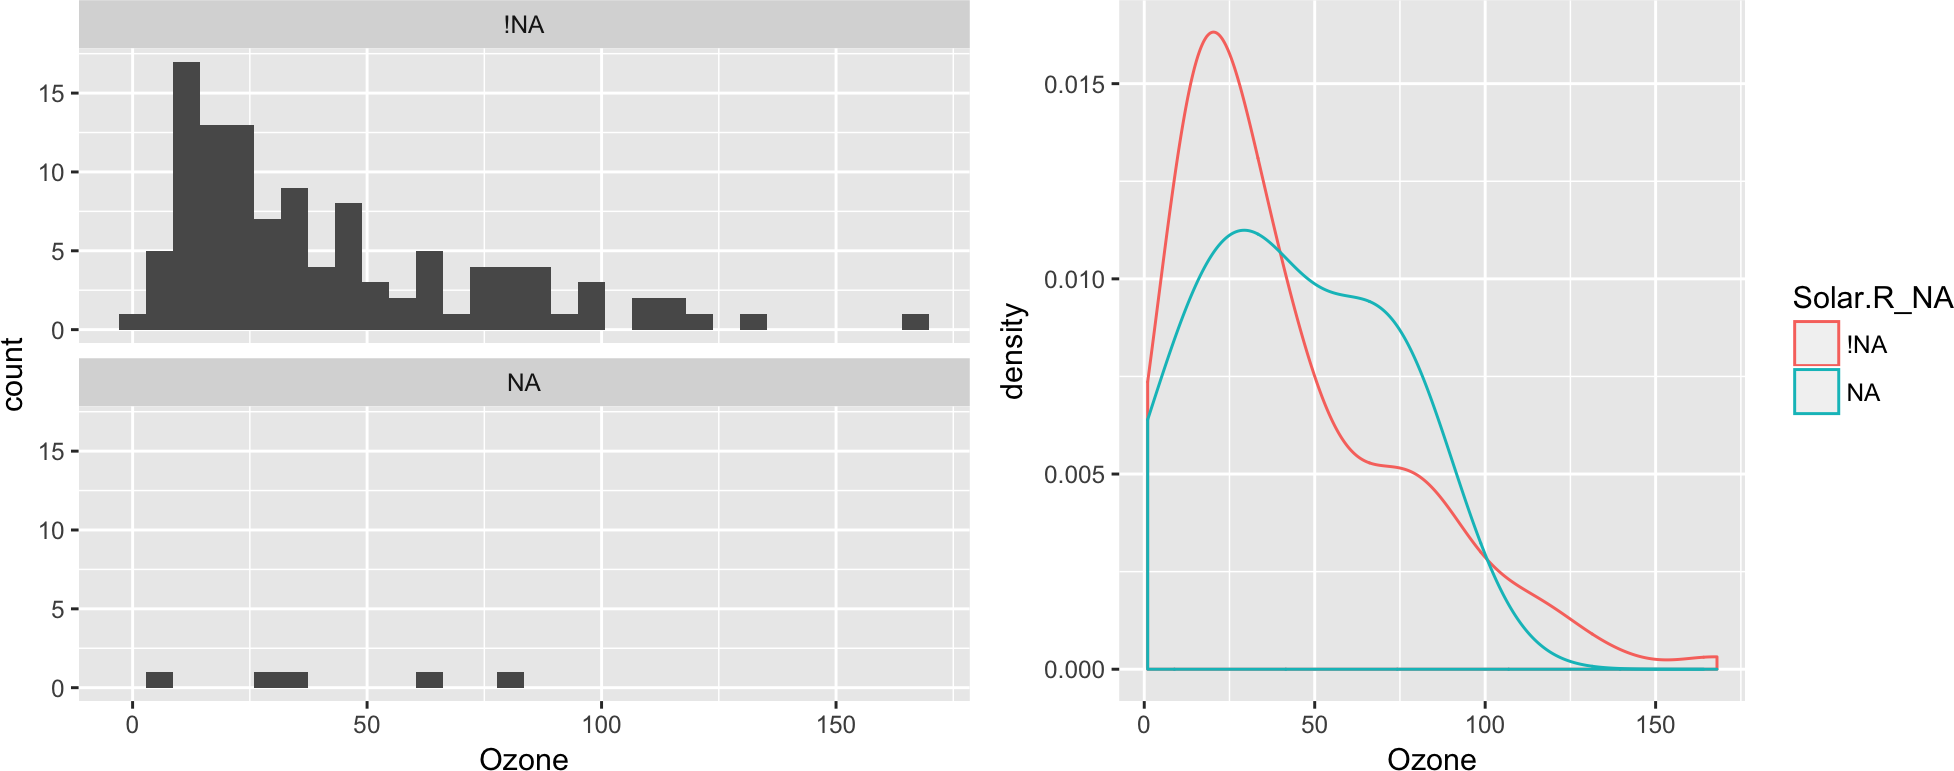
\includegraphics{jsm2017_files/figure-latex/bind-shadow-density-1.png}

Using this data structure facilitates missing data visualisation with
ggplot as it means that the user can directly refer to the variable that
they want to explore missingness. In the case above, the user is looking
at a histogram of Ozone, but is then able to look at how many Ozone
values are affected by Solar.R. In cases where there is no missing data
in the variable that they want to ``split'' the missingness by, the plot
simple returns a single facetted plot.

Another method of visualisation can be explored using
\texttt{geom\_missing\_point()} from the \texttt{ggmissing} package:

\begin{Shaded}
\begin{Highlighting}[]
\KeywordTok{ggplot}\NormalTok{(}\DataTypeTok{data =} \NormalTok{airquality,}
       \KeywordTok{aes}\NormalTok{(}\DataTypeTok{x =} \NormalTok{Ozone,}
           \DataTypeTok{y =} \NormalTok{Solar.R)) +}\StringTok{ }
\StringTok{  }\KeywordTok{geom_missing_point}\NormalTok{()}
\end{Highlighting}
\end{Shaded}

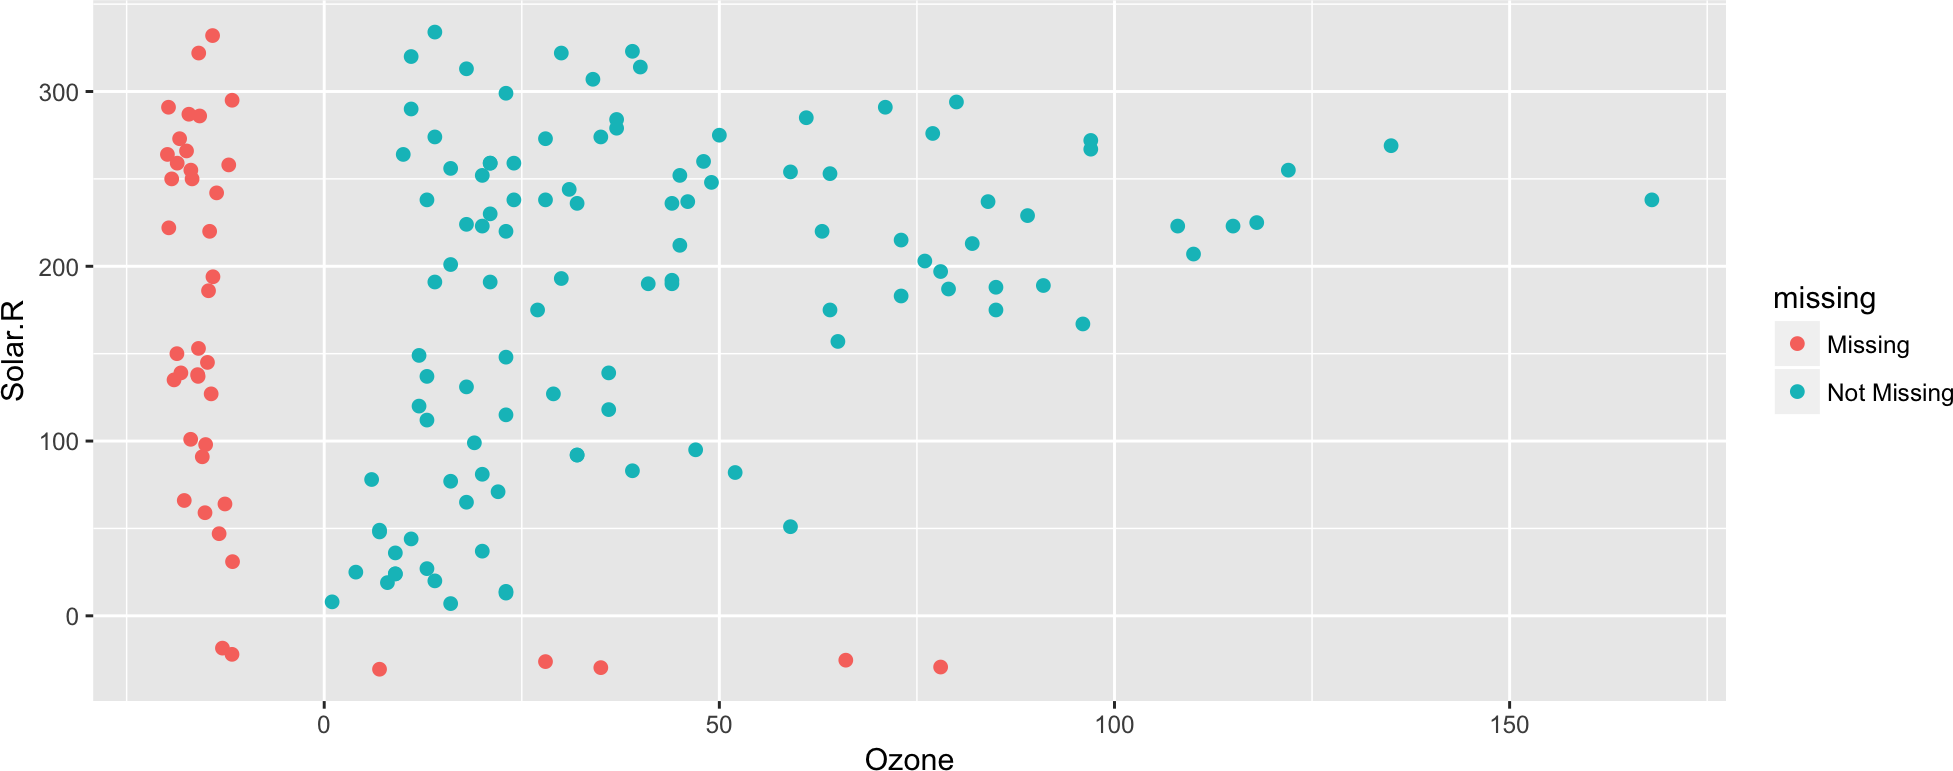
\includegraphics{jsm2017_files/figure-latex/ggeom_missing-1.png}

This replaces missing values to be 10\% below the minimum value, a
technique borrowed from ggobi. The missing values are also different
colours to make missingness preattentive.

\subsection{Numerical Summaries for missing
data}\label{numerical-summaries-for-missing-data}

Numerical summaries of missing data are also made easy with some helper
functions from the \texttt{ggmissing} package. For example, finding the
overall proportion of missing values in the data overall, or the cases,
or variables, can be done with \texttt{percent\_missing\_*} functions.

\begin{Shaded}
\begin{Highlighting}[]
\CommentTok{# Proportion elements in dataset that contains missing values}
\KeywordTok{percent_missing_df}\NormalTok{(airquality)}
\end{Highlighting}
\end{Shaded}

\begin{verbatim}
## [1] 4.793028
\end{verbatim}

\begin{Shaded}
\begin{Highlighting}[]
\CommentTok{# Proportion of variables that contain any missing values}
\KeywordTok{percent_missing_var}\NormalTok{(airquality)}
\end{Highlighting}
\end{Shaded}

\begin{verbatim}
## [1] 33.33333
\end{verbatim}

\begin{Shaded}
\begin{Highlighting}[]
 \CommentTok{# Proportion of cases that contain any missing values}
\KeywordTok{percent_missing_case}\NormalTok{(airquality)}
\end{Highlighting}
\end{Shaded}

\begin{verbatim}
## [1] 27.45098
\end{verbatim}

We can also look at the number and percent of missings in each case, and
in each variable with \texttt{summary\_missing\_case}, and
\texttt{summary\_missing\_var}.

\begin{verbatim}
summary_missing_case(airquality)
\end{verbatim}

\begin{verbatim}
## # A tibble: 5 × 3
##    case n_missing  percent
##   <int>     <int>    <dbl>
## 1     1         0  0.00000
## 2     2         0  0.00000
## 3     3         0  0.00000
## 4     4         0  0.00000
## 5     5         2 33.33333
\end{verbatim}

\begin{Shaded}
\begin{Highlighting}[]
\KeywordTok{summary_missing_var}\NormalTok{(airquality)}
\end{Highlighting}
\end{Shaded}

\begin{verbatim}
## # A tibble: 6 × 3
##   variable n_missing   percent
##      <chr>     <int>     <dbl>
## 1    Ozone        37 24.183007
## 2  Solar.R         7  4.575163
## 3     Wind         0  0.000000
## 4     Temp         0  0.000000
## 5    Month         0  0.000000
## 6      Day         0  0.000000
\end{verbatim}

We can also present tabulations that present more complicated inferences
with \texttt{table\_missing\_case} and \texttt{table\_missing\_var}.
These tally up the number of missings in each case or variable, then
describe how many cases or variables have that many missings, and the
percentage of cases or variables that contain missings

\begin{Shaded}
\begin{Highlighting}[]
\NormalTok{ggmissing::}\KeywordTok{table_missing_case}\NormalTok{(airquality)}
\end{Highlighting}
\end{Shaded}

\begin{verbatim}
## # A tibble: 3 × 3
##   n_missing_in_case n_cases  percent
##               <int>   <int>    <dbl>
## 1                 0     111 72.54902
## 2                 1      40 26.14379
## 3                 2       2  1.30719
\end{verbatim}

\begin{Shaded}
\begin{Highlighting}[]
\NormalTok{ggmissing::}\KeywordTok{table_missing_var}\NormalTok{(airquality)}
\end{Highlighting}
\end{Shaded}

\begin{verbatim}
## # A tibble: 3 × 3
##   n_missing_in_var n_vars  percent
##              <int>  <int>    <dbl>
## 1                0      4 66.66667
## 2                7      1 16.66667
## 3               37      1 16.66667
\end{verbatim}

\section{Discussion}\label{discussion}

We describe the current packages and software for exploring and
visualising missing data.

This is the \texttt{bind\_shadow} versus computing on the fly with
\texttt{is\_na}

\begin{verbatim}

ggplot(data = bind_shadow(airquality),
       aes(x = Ozone)) + 
  geom_histogram() + 
  facet_wrap(Solar.R_NA),
             ncol = 1)
             
ggplot(data = airquality,
       aes(x = Ozone)) + 
  geom_histogram() + 
  facet_wrap(is_na(Solar.R),
             ncol = 1)
\end{verbatim}

It is important to consider then the implications for storage, when
using bind\_shadow, and computation, when using the \texttt{is\_na}
approach. \texttt{bind\_shadow} provides some flexibility and
extensibility, as it allows for more complex types of missingness. For
example, it could extending from missing, \texttt{NA},and not missing,
\texttt{!NA}, to extend to different mechanisms for missingness
\texttt{NA\_missing\_for\_reason\_A},
\texttt{NA\_missing\_for\_reason\_B}, or imputed values
\texttt{value\_imputed}.

\textbf{Limitations}

More research is needed to be done on how to visualise, store, and
summarise imputations while staying in a tidy data framework. Multiple
imputation could be stored using nested dataframes for each multiple
imputation. We didn't discuss how to visualise imputations, but you can
imagine a similar framework for labelling imputations in a data
structure.

\textbf{Future work}

explore model-based approaches for exploring based missing data
structures.

\begin{itemize}
\tightlist
\item
  How does this expand the field?
\item
  How is this different to previous findings / usage?
\end{itemize}

\section*{References}\label{references}
\addcontentsline{toc}{section}{References}

\hypertarget{refs}{}
\hypertarget{ref-cheng2015}{}
Cheng, Xiaoyue, Dianne Cook, Heike Hofmann, and others. 2015. ``Visually
Exploring Missing Values in Multivariable Data Using a Graphical User
Interface.'' \emph{Journal of Statistical Software} 68 (1). Foundation
for Open Access Statistics: 1--23.

\hypertarget{ref-Little1988}{}
Little, Roderick JA. 1988. ``A Test of Missing Completely at Random for
Multivariate Data with Missing Values.'' \emph{Journal of the American
Statistical Association} 83 (404). Taylor \& Francis: 1198--1202.

\hypertarget{ref-Rubin1976}{}
Rubin, Donald B. 1976. ``Inference and Missing Data.'' \emph{Biometrika}
63 (3). Biometrika Trust: 581--92.

\hypertarget{ref-Schafer2002}{}
Schafer, Joseph L., and John W. Graham. 2002. ``Missing data: Our view
of the state of the art.'' \emph{Psychological Methods} 7 (2): 147--77.
doi:\href{https://doi.org/10.1037//1082-989X.7.2.147}{10.1037//1082-989X.7.2.147}.

\hypertarget{ref-simon-simonoff}{}
Simon, Gary A., and Jeffrey S Simonoff. 1986. ``Diagnostic Plots for
Missing Data in Least Squares Regression.'' \emph{Journal of the
American Statistical Association} 81 (394). Taylor \& Francis Group:
501--9.

\hypertarget{ref-Swayne1998}{}
Swayne, Deborah F, and Andreas Buja. 1998. ``Missing Data in Interactive
High-Dimensional Data Visualization.'' \emph{Computational Statistics}
13 (1). Citeseer: 15--26.

\hypertarget{ref-swayne2003ggobi}{}
Swayne, Deborah F, Duncan Temple Lang, Andreas Buja, and Dianne Cook.
2003. ``GGobi: Evolving from Xgobi into an Extensible Framework for
Interactive Data Visualization.'' \emph{Computational Statistics \& Data
Analysis} 43 (4). Elsevier: 423--44.

\hypertarget{ref-vim}{}
Templ, Matthias, Andreas Alfons, Alexander Kowarik, and Bernd Prantner.
2011. ``VIM: Visualization and Imputation of Missing Values.'' \emph{R
Package Version} 2 (3).

\hypertarget{ref-Unwin1996}{}
Unwin, Antony, George Hawkins, Heike Hofmann, and Bernd Siegl. 1996.
``Interactive Graphics for Data Sets with Missing Values - Manet.''
\emph{Journal of Computational and Graphical Statistics} 5 (2). Taylor
\& Francis Group: 113--22.

\hypertarget{ref-Wickham2014}{}
Wickham, Hadley. 2014. ``Tidy Data.'' \emph{J. Stat. Softw.} 59 (1):
1--23.


\end{document}
